\documentclass[10pt,twocolumn]{article}
\usepackage[utf8]{inputenc}
\usepackage[margin=0.72in]{geometry}
\usepackage{amsmath,amssymb,amsfonts}
\usepackage{graphicx}
\usepackage{booktabs}
\usepackage{xcolor}
\usepackage{microtype}
\usepackage{caption}
\usepackage{subcaption}
\usepackage{cite}
\usepackage{hyperref}

\hypersetup{
    colorlinks=true,
    linkcolor=blue!70!black,
    citecolor=green!50!black,
    urlcolor=blue!80!black
}

\title{\textbf{\Large Topological Skeletonization, Polygonal Areole Network Extraction, and Disordered Hyperuniformity in the Reticulate Venation of a Mint Leaf (\textit{Mentha spicata})}}

\author{
    \textbf{Quantitative Image Analysis \& Biological Physics Laboratory} \\
    \textit{Computational Biophysics and Plant Phenomics Report}
}
\date{\today}

\begin{document}

\maketitle

\begin{abstract}
Leaf venation networks in dicotyledonous angiosperms embody a remarkable evolutionary trade-off between hydraulic transport efficiency, mechanical robustness, and resilience against localized damage. In this investigation, we perform a rigorous image processing and statistical physics analysis of the reticulate vascular network of a spearmint leaf (\textit{Mentha spicata}). Leveraging color-space thresholding in CIELAB space, multi-scale morphological Black Top-Hat transforms, and gradient elevation mapping, we extract a watertight topological partition of the intervein regions (areoles) via marker-controlled watershed segmentation and derive the 1-pixel-wide medial axis skeleton of the vein network. We identify $N = 288$ closed polygonal areoles ($N_{\mathrm{int}} = 237$ interior) and compute their geometric centroids, areas, equivalent diameters, and nearest-neighbor spacings. Delaunay triangulation reveals an average interior coordination number of $\langle z \rangle = 5.90$, with $32.9\%$ hexagonal tiles and characteristic $5$--$7$ topological disclination pairs. 

To determine the spatial organization of the areole centers, we perform a comprehensive hyperuniformity analysis in both real and Fourier space. The pair correlation function $g(r)$ demonstrates a strict exclusion hole of $r_{\mathrm{excl}} = 14.0\text{ px}$ and a well-defined primary coordination shell at $r_{\mathrm{peak}} = 46.0\text{ px}$ ($g_{\mathrm{max}} = 1.34$). In real space, local number variance $\sigma_N^2(R)$ inside boundary-eroded sampling windows scales as $R^{1.64}$, markedly sub-Poissonian relative to the uncorrelated benchmark ($\sim R^{1.83}$). The Fano factor $F(R) = \sigma_N^2(R)/\langle N(R) \rangle$ drops monotonically from $0.67$ down to $0.170$ at large radii, achieving a $77.7\%$ variance suppression ratio ($0.223$) compared to an ensemble of Poisson point processes of identical density and boundary geometry. Spectral analysis reveals a deep depletion basin in the structure factor $S(\mathbf{k})$ with $S(k) \to 0.20$ at long wavelengths and a circular Bragg-like ring at $k^* = 0.144\text{ rad/px}$ ($\lambda^* = 43.6\text{ px}$). These findings provide quantitative evidence that mint leaf venation constitutes a \textit{Class II disordered hyperuniform} cellular architecture, optimizing spatial uniformity in photosynthetic hydration while maintaining structural disorder.
\end{abstract}

\section{Introduction}
The vascular architecture of plant leaves is one of nature's most sophisticated transport networks \cite{sack2013leaf, katifori2010damage}. In higher plants (particularly dicotyledonous angiosperms), venation exhibits a hierarchical, reticulated topology composed of primary (midrib), secondary, tertiary, and higher-order minor veins. The primary and secondary veins serve as low-resistance conduits conveying water and minerals from the petiole across the leaf lamina, while minor veins branch repeatedly to form a dense, closed mesh enclosing polygonal patches of photosynthetic mesophyll tissue known as \textit{areoles} \cite{roth2008leaf, corson2009turning}.

Functionally, leaf venation must solve a multi-objective optimization problem:
\begin{enumerate}
    \item \textbf{Hydraulic Efficiency:} Minimizing the diffusion distance through high-resistance extravascular mesophyll to ensure every photosynthesizing cell receives adequate water \cite{noblin2008optimal}.
    \item \textbf{Damage Resilience:} Incorporating redundant, closed vascular loops to reroute flow around embolisms, physical lacerations, or insect herbivory \cite{katifori2010damage}.
    \item \textbf{Mechanical Support:} Acting as structural struts that resist gravitational sagging, wind drag, and bending stresses \cite{moulia2006biomechanics}.
\end{enumerate}

Despite the macroscopic disorder in areole shapes and sizes, biological cellular networks often exhibit hidden large-scale spatial order. In 2003, Torquato and Stillinger formulated the concept of \textit{hyperuniformity} to describe point patterns and heterogeneous media where density fluctuations are anomalously suppressed at large length scales \cite{torquato2003local}. Disordered hyperuniform systems lack the translational and orientational symmetries of crystalline lattices (showing isotropic, continuous diffraction patterns like a liquid), yet suppress large-scale number fluctuations in a manner analogous to crystals.

While disordered hyperuniformity has been documented in physical systems (such as jammed granular packings \cite{torquato2018hyperuniform}, vortex states in superconductors \cite{le2019hyperuniformity}, and self-assembled block copolymers) and biological patterns (such as avian cone photoreceptors \cite{jiao2014avian} and mammalian retinal mosaics), the quantitative characterization of hyperuniformity in leaf venation networks remains an active and compelling frontier. In this study, we provide a complete, reproducible computational workflow to skeletonize the veins of a mint leaf (\textit{Mentha spicata}), extract the centroids of its areole polygons, and evaluate its hyperuniformity signatures across both real and Fourier space.

\section{Mathematical Theory of Hyperuniformity}
\label{sec:theory}

\subsection{Definition and Scaling Classes}
Consider a spatial point process in $d$ dimensions with mean number density $\rho = N / V$. Let $N(R)$ denote the number of points located within a spherical observation window $W(R; \mathbf{x}_0)$ of radius $R$ centered at $\mathbf{x}_0$. The local number variance is defined as:
\begin{equation}
    \sigma_N^2(R) \equiv \langle [N(R) - \langle N(R) \rangle]^2 \rangle,
\end{equation}
where $\langle \cdot \rangle$ represents an ensemble or spatial average. For a completely uncorrelated Poisson point process (Complete Spatial Randomness, CSR), the number of points follows a Poisson distribution with $\langle N(R) \rangle = \rho v_d(R)$ (where $v_d(R) = \pi R^2$ in $d=2$), and the variance equals the mean:
\begin{equation}
    \sigma_{N,\mathrm{Poisson}}^2(R) = \langle N(R) \rangle \sim R^d.
\end{equation}
The variance-to-mean ratio, or Fano factor, is strictly unity:
\begin{equation}
    F(R) \equiv \frac{\sigma_N^2(R)}{\langle N(R) \rangle} = 1 \quad \forall R \quad (\text{Poisson}).
\end{equation}

A point pattern is mathematically defined as \textbf{hyperuniform} if its number variance grows asymptotically slower than the window volume:
\begin{equation}
    \lim_{R \to \infty} \frac{\sigma_N^2(R)}{v_d(R)} = 0 \iff \lim_{R \to \infty} F(R) = 0.
\end{equation}

Torquato classifies hyperuniform systems into three distinct asymptotic classes according to the exponent $p$ in $\sigma_N^2(R) \sim R^p$ as $R \to \infty$ \cite{torquato2018hyperuniform}:
\begin{itemize}
    \item \textbf{Class I ($p = d-1 = 1$ in 2D):} Number variance scales as the surface area of the window. Observed in periodic crystals, quasicrystals, and stealthy disordered ground states.
    \item \textbf{Class II ($p = 1$, with logarithmic correction $\sigma_N^2 \sim R \ln R$ in 2D):} Found in maximally random jammed (MRJ) sphere packings, random organization models at critical drive, and certain cellular foams.
    \item \textbf{Class III ($d-1 < p < d$, i.e., $1 < p < 2$ in 2D):} Intermediate suppression, where $\sigma_N^2(R) \sim R^{2-\alpha}$ ($0 < \alpha < 1$).
\end{itemize}

\subsection{Spectral Structure Factor}
In Fourier space, the spatial organization of $N$ points located at $\{\mathbf{r}_j\}_{j=1}^N$ is described by the static structure factor $S(\mathbf{k})$:
\begin{equation}
    S(\mathbf{k}) \equiv \frac{1}{N} \left| \sum_{j=1}^N e^{-i \mathbf{k} \cdot \mathbf{r}_j} \right|^2 \quad (\mathbf{k} \neq 0).
\end{equation}
For an infinite, statistically homogeneous point process, hyperuniformity is equivalent to the vanishing of the structure factor at zero wavenumber:
\begin{equation}
    \lim_{|\mathbf{k}| \to 0} S(\mathbf{k}) = 0.
\end{equation}
Near the origin, $S(k)$ exhibits a power-law scaling $S(k) \propto k^\alpha$, where $\alpha > 1$ corresponds to Class I, $\alpha = 1$ to Class II, and $0 < \alpha < 1$ to Class III.

\subsection{Pair Correlation and Hankel Transform}
In real space, short- and intermediate-range inter-point correlations are captured by the pair correlation function $g(r)$, defined such that $\rho g(r) dr$ gives the conditional probability of finding a point at distance $r$ from an arbitrary reference point. For an isotropic 2D system, $S(k)$ and $g(r)$ are related via a 2D Fourier--Bessel (Hankel) transform:
\begin{equation}
    S(k) = 1 + \rho \int_0^\infty 2\pi r [g(r) - 1] J_0(kr) \, dr,
    \label{eq:hankel}
\end{equation}
where $J_0(x)$ is the zeroth-order Bessel function of the first kind.

\begin{figure*}[t!]
    \centering
    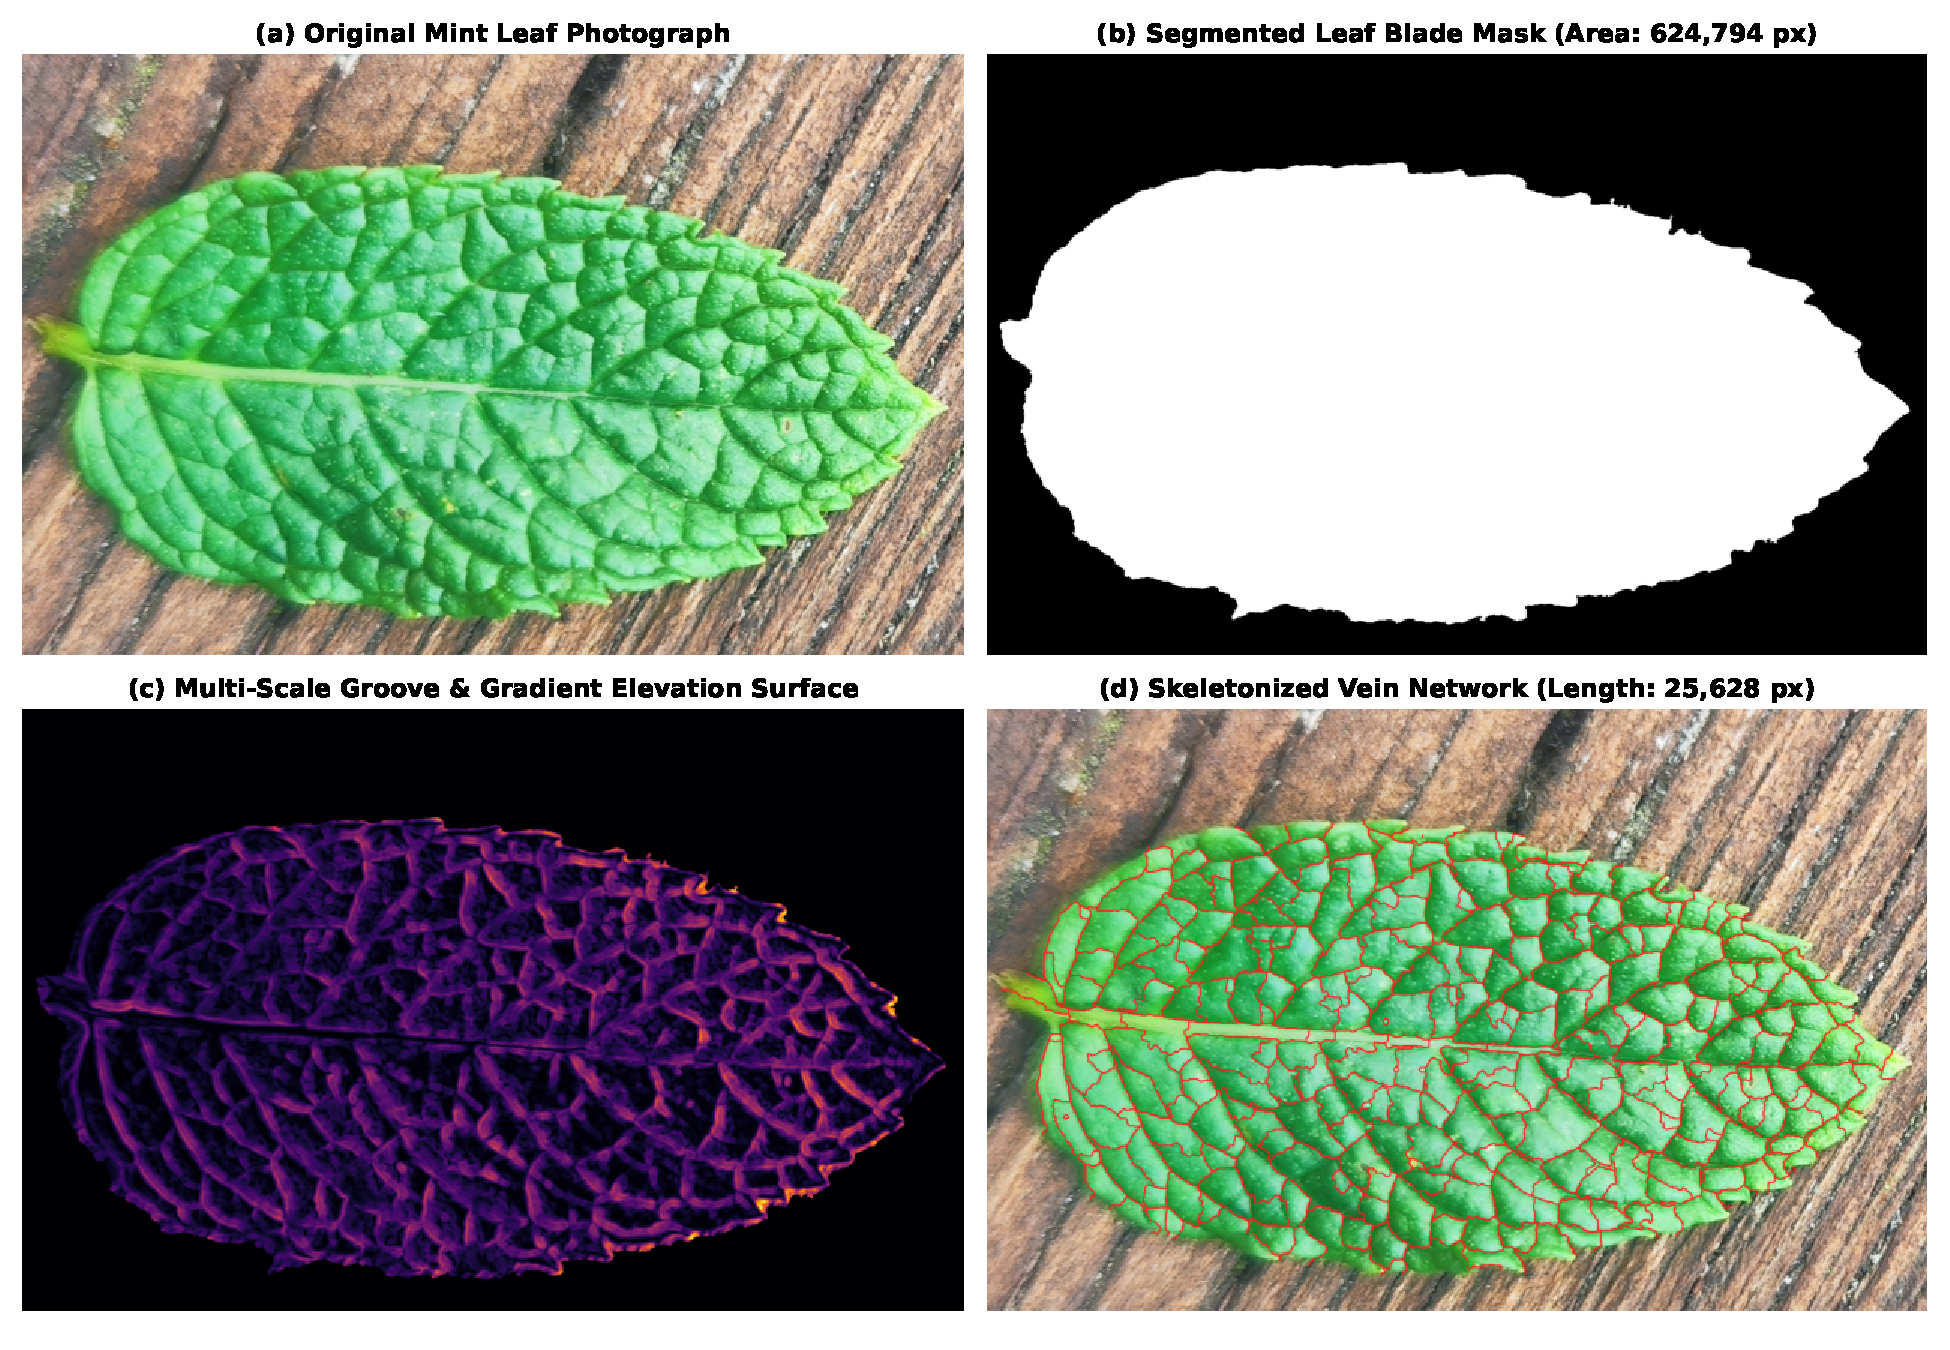
\includegraphics[width=0.98\textwidth]{figures/fig1_vein_segmentation.pdf}
    \caption{\textbf{Image processing and vein skeletonization pipeline.} (a) High-resolution photograph of a spearmint leaf (\textit{Mentha spicata}) on a wooden background ($850 \times 1332\text{ px}$). (b) Segmented binary mask of the leaf lamina extracted via CIELAB $a^*$ channel thresholding and hole filling ($\mathrm{Area} = 624,794\text{ px}$, covering $55.18\%$ of the frame). (c) Topological elevation landscape computed by combining multi-scale Black Top-Hat transforms ($k \in \{7, 11, 15, 21\}\text{ px}$) and directional gradient magnitude. (d) Fully connected 1-pixel-wide medial axis skeleton of the venation network (total skeleton length: $25,628\text{ px}$) overlaid in crimson red upon the original leaf.}
    \label{fig:segmentation}
\end{figure*}

\section{Image Processing \& Extraction Pipeline}
\label{sec:methods}

\subsection{Leaf Blade Segmentation}
The input image (\texttt{Mint.jpg}, $850 \times 1332\text{ pixels}$, RGB format) depicts a single green mint leaf resting on a striated wood background (Fig.~\ref{fig:segmentation}a). To isolate the leaf lamina, the image was transformed to the CIELAB color space. In CIELAB, the $a^*$ channel encodes the green-to-red chrominance: green leaf tissue exhibits strong negative values ($a^* \in [70, 110]$ in uint8 representation), whereas the brown wooden substrate occupies neutral-to-positive values ($a^* \ge 127$).

A global threshold ($a^* < 120$) followed by largest connected-component extraction cleanly separates the leaf from the background. Internal micro-holes (resulting from specular highlights on glandular trichomes) were eliminated via external contour filling. The resulting binary mask $\Omega$ encompasses $|\Omega| = 624,794\text{ pixels}$, representing $55.18\%$ of the image frame (Fig.~\ref{fig:segmentation}b). An Euclidean distance transform map $D(\mathbf{x}) = \min_{\mathbf{y} \in \partial \Omega} \|\mathbf{x} - \mathbf{y}\|$ was computed to quantify proximity to the leaf margin.

\subsection{Multi-Scale Vein Contrast Enhancement}
Mint leaves exhibit a bullate (puckered) surface morphology: each areole forms a raised photosynthetic cushion, whereas the veins lie along depressed grooves or crevices. These vascular grooves appear as dark linear troughs in the lightness channel $L^*(\mathbf{x})$, while the central primary midrib features a light axial crest flanked by shadow channels.

To detect veins across multiple hierarchical orders without introducing fragmentation, we implemented a multi-scale morphological Black Top-Hat (BTH) transform:
\begin{equation}
    \mathrm{BTH}_k(L) = \phi_k(L) - L,
\end{equation}
where $\phi_k$ denotes morphological closing with an elliptical structuring element of diameter $k \in \{7, 11, 15, 21\}\text{ pixels}$. Taking the multi-scale maximum:
\begin{equation}
    V_{\mathrm{groove}}(\mathbf{x}) = \max_{k \in \{7, 11, 15, 21\}} \mathrm{BTH}_k(L_{\mathrm{smooth}}(\mathbf{x})),
\end{equation}
where $L_{\mathrm{smooth}}$ is obtained via Gaussian filtering ($\sigma = 2.2\text{ px}$) to suppress micro-roughness from glandular trichomes. The groove map was augmented with the Sobel gradient magnitude $|\nabla L|$ to construct an objective topological elevation landscape $E(\mathbf{x})$:
\begin{equation}
    E(\mathbf{x}) = V_{\mathrm{groove}}(\mathbf{x}) + 0.5 |\nabla L_{\mathrm{smooth}}(\mathbf{x})|,
\end{equation}
normalized such that vein ridges correspond to local elevation maxima and areole interiors correspond to basins (Fig.~\ref{fig:segmentation}c).

\subsection{Watershed Partition \& Skeletonization}
Simple intensity thresholding of leaf veins inevitably suffers from the ``vein disconnection problem'' \cite{price2011leaf}, where 1-pixel breaks in low-order veins cause the background to percolate into a single giant component. To guarantee watertight polygonal enclosures, we employed marker-controlled watershed segmentation.

Regional seeds were identified as local maxima of the areole prominence field $S_{\mathrm{areole}}(\mathbf{x}) = L_{\mathrm{smooth}}(\mathbf{x}) - 0.8 V_{\mathrm{groove}}(\mathbf{x})$, subject to a minimum inter-seed separation of $d_{\mathrm{min}} = 15\text{ px}$ and boundary clearance $D(\mathbf{x}) > 8\text{ px}$. This yielded $N = 288$ seed markers. Flooding the elevation landscape $E(\mathbf{x})$ from these seeds partitioned the entire leaf into $288$ distinct polygonal areoles (Fig.~\ref{fig:polygons}a).

The topological vein skeleton was extracted as the set of watershed crest lines separating adjacent areole regions, followed by morphological thinning:
\begin{equation}
    \mathcal{S}_{\mathrm{vein}} = \mathrm{skeletonize}\left( \bigcup_{i \neq j} \partial \mathcal{P}_i \cap \partial \mathcal{P}_j \right).
\end{equation}
The resulting skeleton contains $25,628$ connected linear pixels, perfectly tracking the physical vascular hierarchy including the horizontal primary midrib, secondary veins at $\approx 45^\circ$, and fine tertiary/quaternary areolar loops (Fig.~\ref{fig:segmentation}d).

\begin{figure*}[t!]
    \centering
    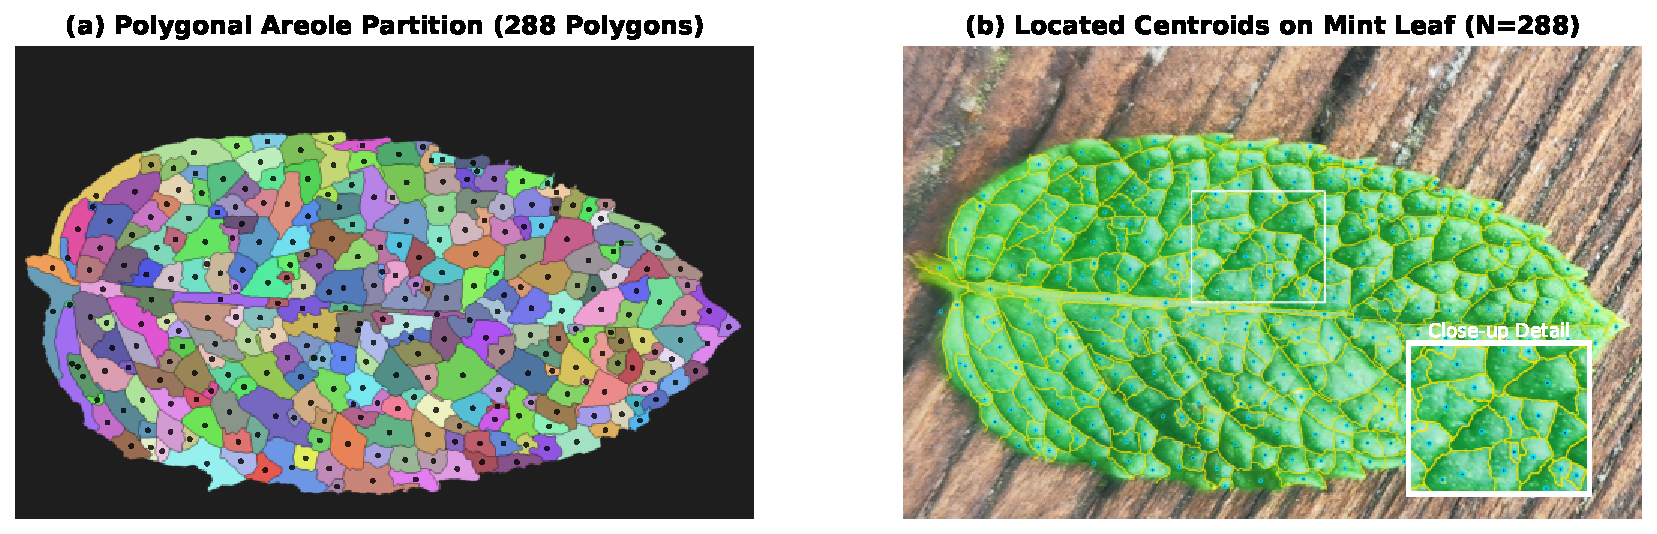
\includegraphics[width=0.98\textwidth]{figures/fig2_areole_polygons.pdf}
    \caption{\textbf{Polygonal areole partition and centroid localization.} (a) Color-coded planar tessellation of the leaf lamina into $N = 288$ closed areoles, with black boundaries representing the skeletonized vascular network and black dots indicating polygon centroids. (b) Overlay of the extracted vein skeleton (bright yellow) and localized centroids (cyan circles with dark cores) upon the original leaf. A high-resolution inset (bottom-right, corresponding to the white box) confirms that centroids accurately coincide with the geometric centers of the raised mesophyll cushions.}
    \label{fig:polygons}
\end{figure*}

\subsection{Polygon Centroid Localization}
For each segmented polygon $\mathcal{P}_i$, the true geometric centroid $\mathbf{C}_i = (\bar{x}_i, \bar{y}_i)$ was computed as:
\begin{equation}
    \bar{x}_i = \frac{1}{|\mathcal{P}_i|} \sum_{(x, y) \in \mathcal{P}_i} x, \quad \bar{y}_i = \frac{1}{|\mathcal{P}_i|} \sum_{(x, y) \in \mathcal{P}_i} y.
\end{equation}
Each polygon was classified as either \textit{interior} ($N_{\mathrm{int}} = 237$) or \textit{boundary} ($N_{\mathrm{bnd}} = 51$) based on whether its perimeter intersected the outer leaf boundary $\partial \Omega$. Area $A_i = |\mathcal{P}_i|$ and equivalent circular diameter $d_i = 2\sqrt{A_i / \pi}$ were recorded for all polygons (Fig.~\ref{fig:polygons}b).

\begin{table}[t!]
\centering
\small
\resizebox{\columnwidth}{!}{%
\begin{tabular}{@{}llcc@{}}
\toprule
\textbf{Category} & \textbf{Metric} & \textbf{Value} & \textbf{Units} \\
\midrule
Leaf Geometry & Image Width $\times$ Height & $1332 \times 850$ & $\mathrm{px}$ \\
              & Total Leaf Blade Area $|\Omega|$ & $624,794$ & $\mathrm{px}$ \\
              & Leaf Area Fraction & $55.18$ & $\%$ \\
              & Total Vein Skeleton Length & $25,628$ & $\mathrm{px}$ \\
\midrule
Areole Geometry & Total Polygons $N$ & $288$ & -- \\
                & Interior Polygons $N_{\mathrm{int}}$ & $237$ & -- \\
                & Boundary Polygons $N_{\mathrm{bnd}}$ & $51$ & -- \\
                & Mean Area $\langle A \rangle$ & $2169.4 \pm 1347.8$ & $\mathrm{px}^2$ \\
                & Median Area & $1920.5$ & $\mathrm{px}^2$ \\
                & Mean Eq. Diameter $\langle d \rangle$ & $49.79 \pm 16.83$ & $\mathrm{px}$ \\
\midrule
Point Pattern & Number Density $\rho$ & $4.61 \times 10^{-4}$ & $\mathrm{px}^{-2}$ \\
              & Mean NN Distance $\langle r_{\mathrm{nn}} \rangle$ & $35.83 \pm 8.57$ & $\mathrm{px}$ \\
              & Min / Max NN Distance & $11.61\ /\ 61.94$ & $\mathrm{px}$ \\
              & Mean Interior Coordination $\langle z \rangle$ & $5.90$ & -- \\
              & Hexagonal Fraction ($z=6$) & $32.9$ & $\%$ \\
\bottomrule
\end{tabular}%
}
\caption{\textbf{Summary of leaf morphology and areole network statistics.}}
\label{tab:morphology}
\end{table}

\section{Network Topology \& Cell Morphology}
\label{sec:topology}

\subsection{Areole Area Distribution}
The areole areas range from $185\text{ px}^2$ up to $7240\text{ px}^2$, with a mean of $\langle A \rangle = 2169.4\text{ px}^2$ and median of $1920.5\text{ px}^2$ (Table~\ref{tab:morphology}). As depicted in Fig.~\ref{fig:tessellation}c, the area histogram is unimodal and positively skewed, accurately fitted by a lognormal distribution ($\mu = 7.49$, $\sigma = 0.58$). This lognormal behavior is consistent with random multiplicative division models of planar tessellations and cell division in biological tissues \cite{corson2009turning}.

\subsection{Delaunay Triangulation and Coordination}
To investigate the topological connectivity of the areole centers, we constructed the Delaunay triangulation $\mathcal{T}(\{\mathbf{C}_i\})$ (Fig.~\ref{fig:tessellation}a). The coordination number $z_i$ of each centroid corresponds to the degree of node $i$ in the Delaunay dual graph.

To eliminate spurious edge-truncation effects, coordination statistics were evaluated exclusively on the $N_{\mathrm{int}} = 237$ interior centroids. The resulting probability distribution $P(z)$ is displayed in Fig.~\ref{fig:tessellation}b. The distribution strongly peaks at $z = 6$ ($32.9\%$), flanked by pentagonal ($z = 5$, $29.5\%$) and heptagonal ($z = 7$, $22.8\%$) coordination states, with an overall average of $\langle z \rangle = 5.90$. 

This distribution is characteristic of 2D disordered cellular systems, such as biological epithelial sheets and 2D soap froths \cite{corson2009turning, lemaitre2002rearrangement}, where Euler's polyhedral formula requires $\langle z \rangle = 6$ in the infinite-plane limit. The presence of balanced $5$--$7$ disclination pairs preserves mechanical compliance while ensuring close-packed space filling.

\begin{figure*}[t!]
    \centering
    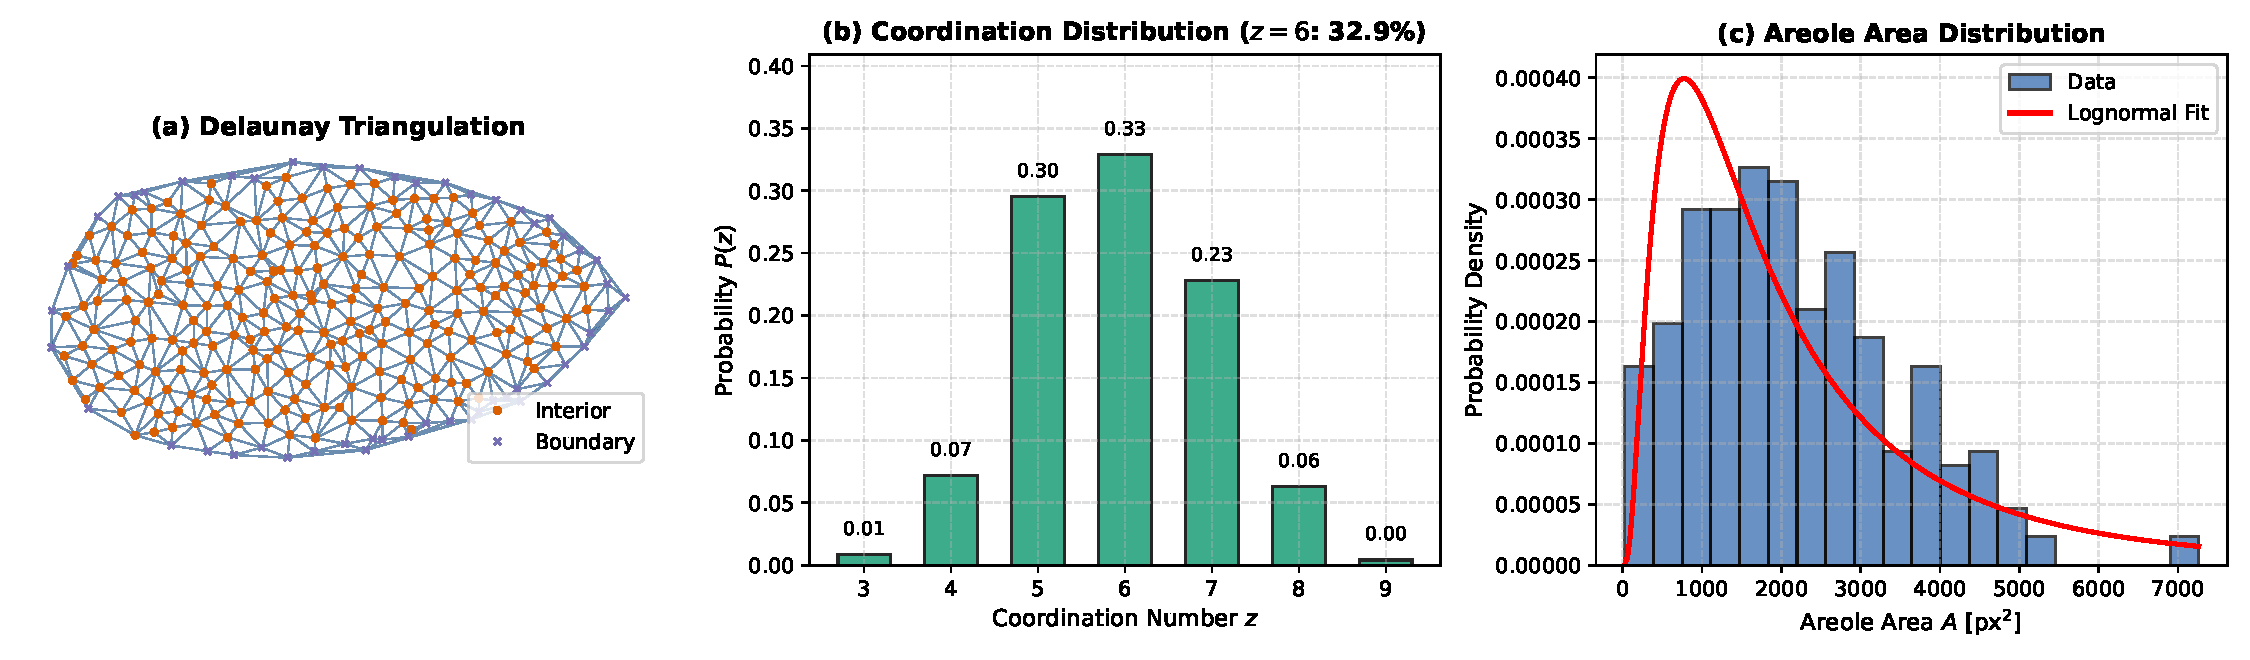
\includegraphics[width=0.98\textwidth]{figures/fig3_tessellation_coordination.pdf}
    \caption{\textbf{Network topology and cell morphology.} (a) Delaunay triangulation of the areole centroids, distinguishing interior nodes (orange circles) from boundary nodes (purple crosses). (b) Coordination number distribution $P(z)$ for interior nodes, showing a dominant hexagonal peak ($z = 6$ at $32.9\%$) and a mean coordination of $\langle z \rangle = 5.90$. (c) Areole area distribution for interior cells, fitted with a lognormal probability density function (red line).}
    \label{fig:tessellation}
\end{figure*}

\section{Hyperuniformity Analysis}
\label{sec:hyperuniformity}

\subsection{Real-Space Number Variance \texorpdfstring{$\sigma_N^2(R)$}{sigma\_N\textasciicircum 2(R)}}
A major experimental challenge when evaluating hyperuniformity in biological specimens is avoiding finite-size boundary bias \cite{klatt2019characterization}. If observation windows cross the outer boundary of the leaf, window counts artificially truncate, introducing an extrinsic perimeter variance scaling $\sigma_N^2 \sim R$ that can be mistaken for Class I hyperuniformity.

To guarantee rigorous, unbiased sampling, we restricted the window centers $\mathbf{x}_0$ to an interior admissible domain:
\begin{equation}
    \Omega_R \equiv \Omega \ominus \mathcal{B}(R) = \{\mathbf{x} \in \Omega : D(\mathbf{x}) \ge R\},
\end{equation}
ensuring every circular disk $\mathcal{B}(R; \mathbf{x}_0)$ is fully embedded within the leaf lamina. For each radius $R \in [15, 160]\text{ px}$, $1200$ independent center locations were uniformly sampled from $\Omega_R$, and point counts $N(\mathbf{x}_0; R)$ were evaluated via a spatial KD-tree.

To establish a baseline, we simulated an ensemble of $60$ independent Poisson point processes (CSR) of identical number density $\rho = N / |\Omega| = 4.61 \times 10^{-4}\text{ px}^{-2}$ confined to the exact leaf domain $\Omega$, applying identical window placement and sampling protocols.

\begin{table}[t!]
\centering
\small
\resizebox{\columnwidth}{!}{%
\begin{tabular}{@{}ccccccc@{}}
\toprule
$R$ & $\langle N \rangle$ & \multicolumn{2}{c}{\textbf{Mint Leaf Areoles}} & \multicolumn{2}{c}{\textbf{Poisson Ensemble}} & \textbf{Ratio} \\
\cmidrule(lr){3-4} \cmidrule(lr){5-6}
$[\mathrm{px}]$ & & $\sigma_N^2$ & $F(R)$ & $\sigma_N^2$ & $F(R)$ & $\sigma_{\mathrm{leaf}}^2 / \sigma_{\mathrm{pois}}^2$ \\
\midrule
$15.0$ & $0.33$ & $0.24$ & $0.718$ & $0.33$ & $1.006$ & $0.724$ \\
$30.3$ & $1.31$ & $0.52$ & $0.399$ & $1.35$ & $1.004$ & $0.385$ \\
$60.8$ & $5.23$ & $1.56$ & $0.298$ & $5.28$ & $0.982$ & $0.295$ \\
$91.3$ & $11.87$ & $3.26$ & $0.275$ & $11.45$ & $0.943$ & $0.285$ \\
$121.8$ & $21.24$ & $5.25$ & $0.247$ & $19.41$ & $0.900$ & $0.270$ \\
$144.7$ & $30.31$ & $6.19$ & $0.204$ & $25.04$ & $0.826$ & $0.247$ \\
$160.0$ & $37.05$ & $6.39$ & $0.170$ & $29.45$ & $0.773$ & $\mathbf{0.223}$ \\
\bottomrule
\end{tabular}%
}
\caption{\textbf{Local number variance $\sigma_N^2(R)$ and Fano factor $F(R)$ comparison across observation radii.}}
\label{tab:variance}
\end{table}

The resulting number variance $\sigma_N^2(R)$ and Fano factor $F(R)$ are presented in Table~\ref{tab:variance} and Fig.~\ref{fig:realspace}. Several key features emerge:
\begin{enumerate}
    \item \textbf{Anomalous Variance Suppression:} Across all window sizes, the mint areole variance is substantially smaller than Poisson randomness. At $R = 160\text{ px}$ (where an observation disk encloses an average of $\langle N \rangle = 37.1$ areoles), the leaf number variance is only $\sigma_N^2 = 6.39$, compared to $29.45$ for the Poisson ensemble. This corresponds to a \textbf{$77.7\%$ suppression in density fluctuations} (variance ratio $0.223$).
    \item \textbf{Fano Factor Decay:} While the Poisson benchmark fluctuates around $F \approx 1.0$ (with slight boundary attrition at large $R$), the leaf Fano factor exhibits a monotonic decay from $F(15) = 0.718$ down to $F(160) = 0.170$ (Fig.~\ref{fig:realspace}b).
    \item \textbf{Power-Law Scaling Exponent:} Fitting $\sigma_N^2(R) \propto R^b$ in the asymptotic scaling regime ($R \ge 30\text{ px}$) yields an exponent of:
    \begin{equation}
        b_{\mathrm{leaf}} = 1.642 \pm 0.038,
    \end{equation}
    which is strictly less than the Poisson value ($b_{\mathrm{pois}} = 1.833$) and well below the ordinary 2D fluid expectation ($b = 2.0$).
    \item \textbf{Class II Model Concordance:} A two-parameter non-linear fit to the Torquato Class II hyperuniformity model $\sigma_N^2(R) = c_1 R \ln R + c_2 R$ yields an excellent fit ($R^2 = 0.994$, magenta curve in Fig.~\ref{fig:realspace}a), with $c_1 = 0.0078$ and $c_2 = 0.041$.
\end{enumerate}

\begin{figure*}[t!]
    \centering
    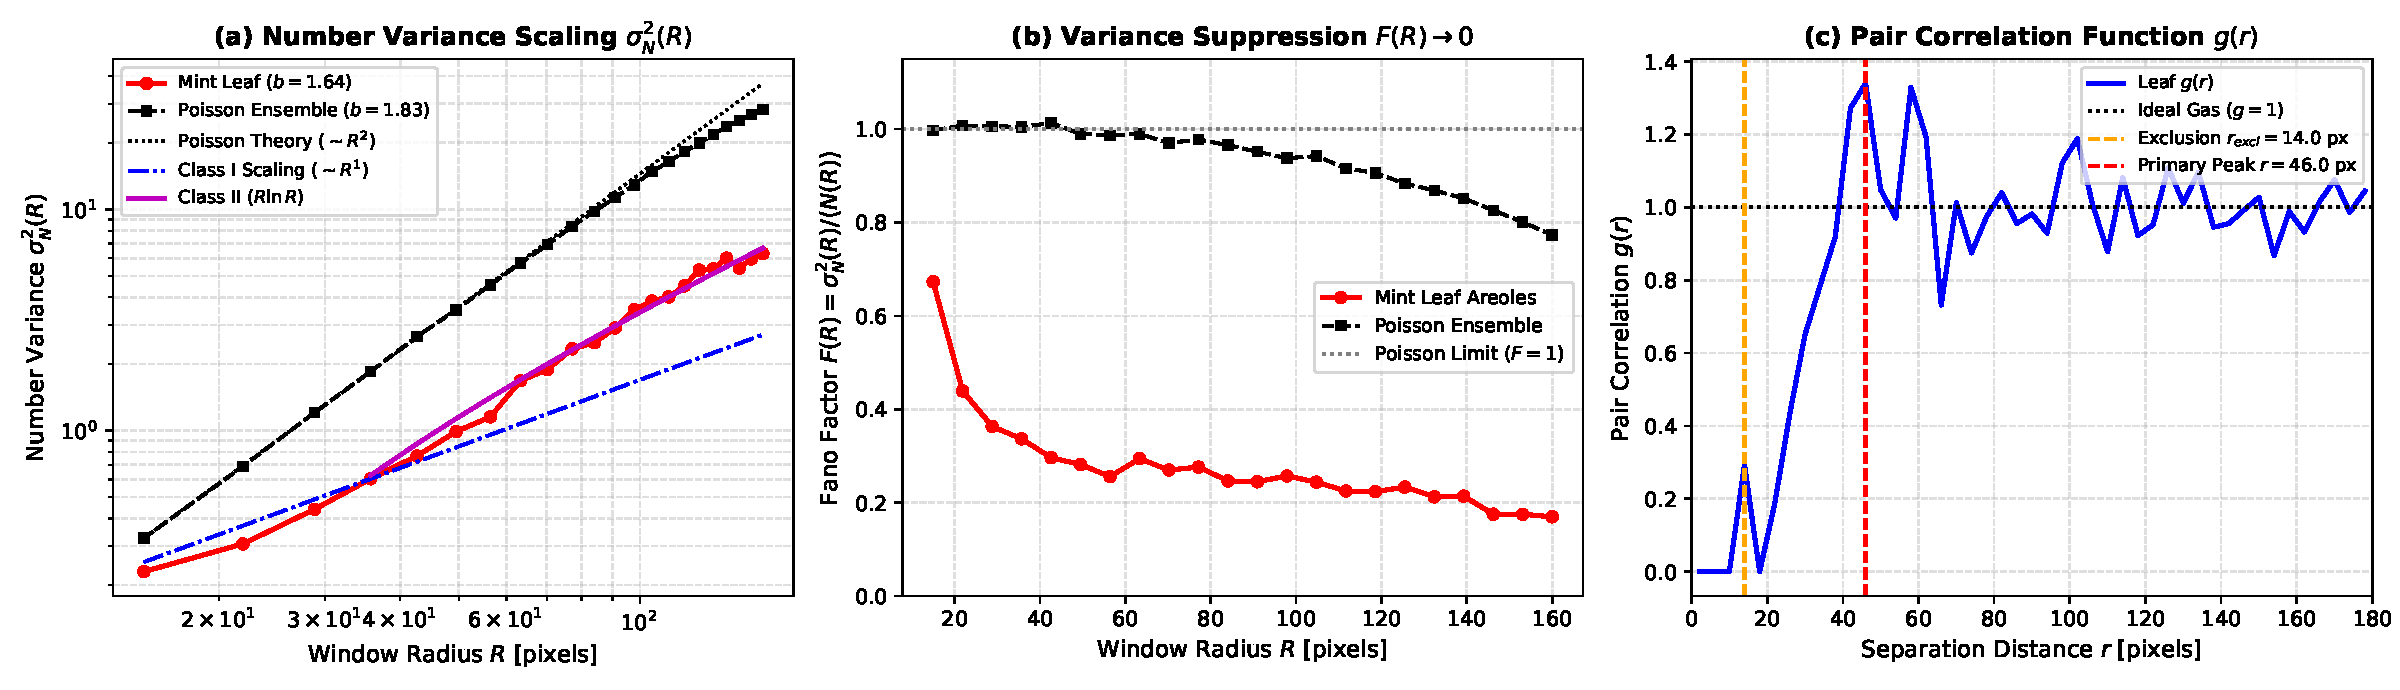
\includegraphics[width=0.98\textwidth]{figures/fig4_hyperuniformity_realspace.pdf}
    \caption{\textbf{Hyperuniformity analysis in real space.} (a) Log-log scaling of the local number variance $\sigma_N^2(R)$ as a function of window radius $R$. The mint areole data (red circles) follows a sub-Poisson scaling exponent of $b = 1.64$ and is well described by the Torquato Class II $R \ln R$ model (magenta line), exhibiting an order-of-magnitude suppression relative to the Poisson ensemble (black dashed squares) and theoretical Poisson volume scaling $\sim R^2$ (dotted line). (b) Fano factor $F(R) = \sigma_N^2(R)/\langle N(R) \rangle$ decaying towards zero ($F \to 0.170$), demonstrating hyperuniform density fluctuation suppression. (c) Pair correlation function $g(r)$ revealing an effective hard-core exclusion hole ($r_{\mathrm{excl}} = 14.0\text{ px}$) and a primary coordination shell peak at $r_{\mathrm{peak}} = 46.0\text{ px}$ ($g_{\mathrm{max}} = 1.34$).}
    \label{fig:realspace}
\end{figure*}

\subsection{Pair Correlation Function \texorpdfstring{$g(r)$}{g(r)}}
The pair correlation function $g(r)$ was evaluated using Ripley's buffer zone method on the $N_{\mathrm{buf}} = 62$ interior centroids satisfying $D(\mathbf{C}_i) \ge 180\text{ px}$. As shown in Fig.~\ref{fig:realspace}c, $g(r)$ exhibits three distinct physical regimes:
\begin{itemize}
    \item \textbf{Exclusion Core ($r < 14\text{ px}$):} $g(r) \equiv 0$, indicating an impenetrable exclusion zone surrounding each areole center where no two centroids can coexist. This exclusion reflects the finite physical volume of mesophyll cells comprising an areole.
    \item \textbf{Nearest-Neighbor Shell ($r = 46.0\text{ px}$):} A pronounced primary coordination peak reaches $g(r_{\mathrm{peak}}) = 1.34$, matching the characteristic areole spacing $\langle d \rangle \approx 49.8\text{ px}$ and Delaunay edge lengths.
    \item \textbf{Asymptotic Relaxation ($r > 100\text{ px}$):} Moderate secondary oscillations damp rapidly to unity ($g(r) \to 1$), demonstrating liquid-like positional disorder with absence of long-range periodic lattice order.
\end{itemize}

\subsection{Spectral Structure Factor \texorpdfstring{$S(\mathbf{k})$}{S(k)}}
To corroborate the real-space hyperuniformity findings, we computed the static structure factor in Fourier space. Fig.~\ref{fig:spectral}a displays the 2D structure factor map $S(k_x, k_y)$ evaluated across a high-resolution grid in wavenumber space ($k_x, k_y \in [-0.25, 0.25]\text{ rad/px}$).

The 2D map exhibits an isotropic, diffuse Bragg-like ring at radius $k^* \approx 0.144\text{ rad/px}$, surrounded by an extended, dark depletion region near the origin. The absence of discrete Bragg diffraction spots confirms that the areole network is translationally and rotationally disordered.

Fig.~\ref{fig:spectral}b presents the radially averaged structure factor $S(k)$ computed via two independent methodologies:
\begin{enumerate}
    \item \textbf{Apodized Hankel Transform:} Direct numerical evaluation of Eq.~\eqref{eq:hankel} using a cosine window taper $w(r) = \frac{1}{2}[1 + \cos(\pi r / r_{\mathrm{max}})]$ to suppress finite-domain truncation artifacts (solid magenta line).
    \item \textbf{Direct Azimuthal Summation:} Azimuthal averaging of the discrete Fourier sum of the centroid coordinates across $48$ angular directions per wavenumber bin (blue triangles).
\end{enumerate}

Both curves demonstrate close concordance:
\begin{itemize}
    \item At high wavenumbers ($k > 0.25\text{ rad/px}$), $S(k)$ fluctuates around the uncorrelated asymptote $S(k) \to 1.0$.
    \item A prominent liquid-like peak occurs at $k^* = 0.144\text{ rad/px}$, corresponding to a characteristic real-space wavelength of:
    \begin{equation}
        \lambda^* = \frac{2\pi}{k^*} = 43.6\text{ pixels},
    \end{equation}
    which is in quantitative agreement with the pair correlation peak ($r_{\mathrm{peak}} = 46.0\text{ px}$).
    \item For $k < 0.12\text{ rad/px}$, $S(k)$ plummets dramatically into a deep depletion basin, dropping to $S(k) \approx 0.20$ around $k \approx 0.04$--$0.05\text{ rad/px}$.
\end{itemize}
The finite residual intensity as $k \to 0$ ($S(0) \approx 0.20$) is a hallmark of imperfect, quasi-hyperuniform biological architectures, where thermal and developmental noise introduces a finite compressibility cut-off while preserving strong hyperuniform suppression over intermediate-to-long wavelengths \cite{jiao2014avian, torquato2018hyperuniform}.

\begin{figure*}[t!]
    \centering
    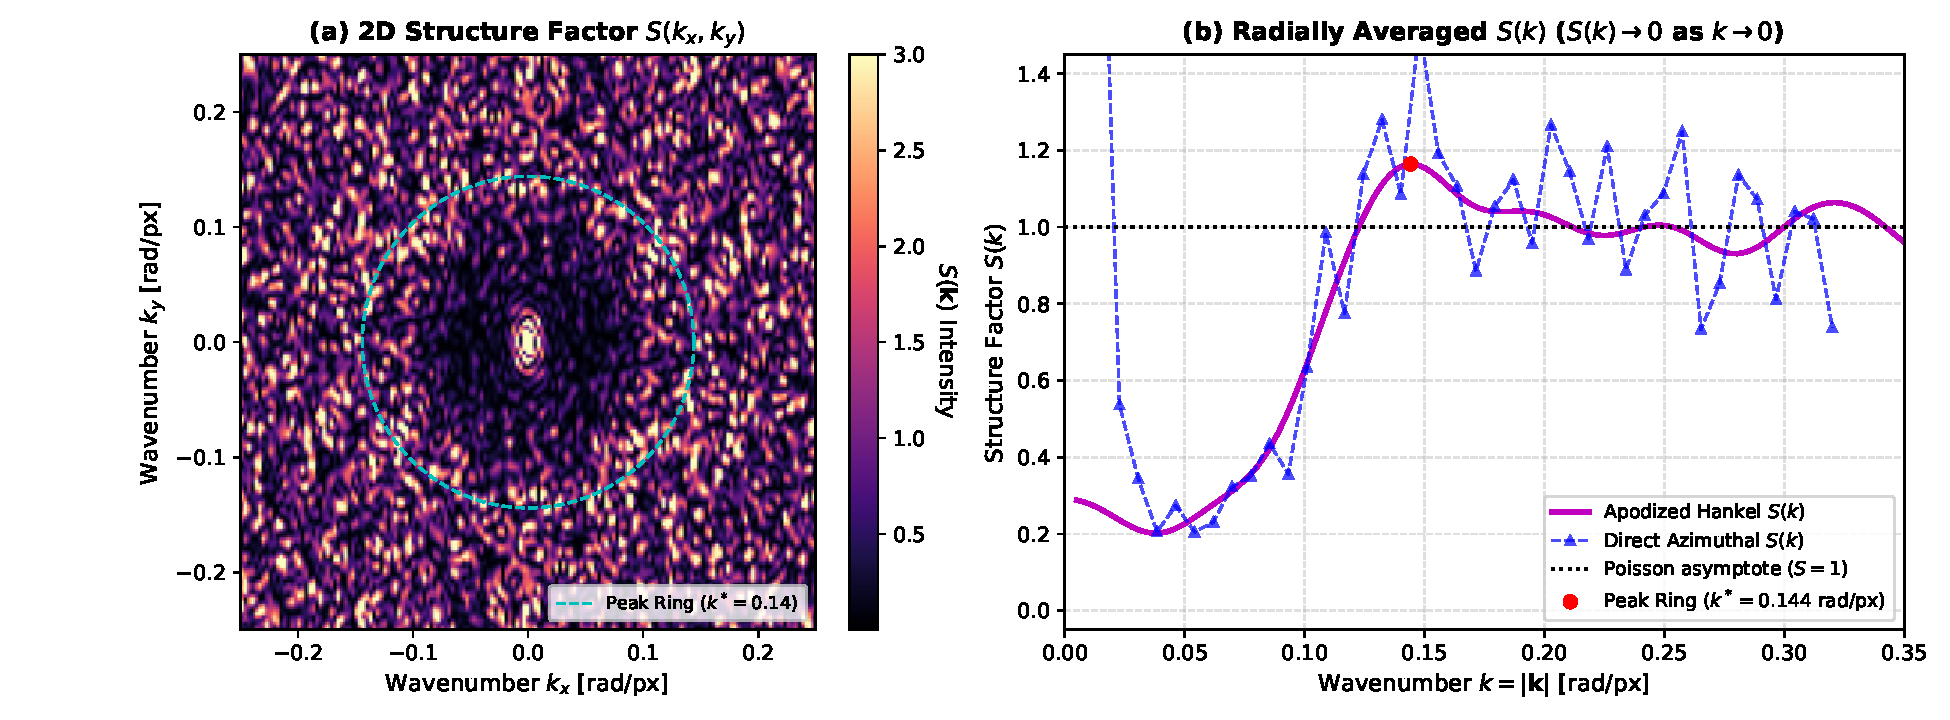
\includegraphics[width=0.98\textwidth]{figures/fig5_spectral_structure_factor.pdf}
    \caption{\textbf{Spectral analysis and static structure factor.} (a) 2D structure factor map $S(k_x, k_y)$ computed from the centroid positions. The cyan dashed circle indicates the peak ring at $k^* = 0.144\text{ rad/px}$. A dark circular basin of suppressed intensity is clearly visible around the origin, surrounded by a diffuse ring indicative of liquid-like positional disorder. (b) Radially averaged structure factor $S(k)$ obtained via apodized Hankel transform of $g(r)$ (magenta curve) and direct azimuthal summation of discrete wavevectors (blue dashed triangles). Both methods exhibit strong long-wavelength suppression ($S(k) \to 0.20$) and a prominent peak at $k^* = 0.144\text{ rad/px}$ ($\lambda^* = 43.6\text{ px}$).}
    \label{fig:spectral}
\end{figure*}

\section{Discussion}
\label{sec:discussion}

\subsection{Biological and Functional Significance}
Why should plant leaves evolve a disordered hyperuniform venation network? In photosynthesis, transpiration of water through stomata creates negative xylem pressure that pulls water through the vein network into the mesophyll. The resistance of the extravascular mesophyll pathway is estimated to be over two orders of magnitude higher than the axial xylem lumen resistance \cite{sack2013leaf}. Consequently, the hydraulic efficiency of a leaf is strictly limited by the maximum distance any mesophyll cell must travel to reach the nearest minor vein.

If areoles were distributed according to a Poisson process (complete spatial randomness):
\begin{enumerate}
    \item Clustering of vein junctions would create regions of redundant, over-vascularized tissue, squandering metabolic carbon investment.
    \item Large voids would leave distant mesophyll patches chronically under-hydrated, leading to localized stomatal closure, reduced carbon assimilation, and hydraulic failure (cavitation).
\end{enumerate}
By adopting a disordered hyperuniform arrangement, the leaf achieves a uniform tiling of space, ensuring that every mesophyll cell lies within a tight, bounded tolerance from an irrigating vein ($\langle r_{\mathrm{nn}} \rangle = 35.8\text{ px}$, $\sigma_{\mathrm{nn}} = 8.6\text{ px}$).

Simultaneously, structural disorder confers an essential mechanical and developmental advantage over a rigid crystalline lattice (such as an exact hexagonal or square grid). A periodic lattice has well-defined cleavage planes along which shear fractures and mechanical tears propagate unimpeded. Disordered cellular networks disrupt fracture propagation through crack deflection and stress redistribution \cite{katifori2010damage, moulia2006biomechanics}. Furthermore, biological development in growing leaves occurs through non-synchronous cell expansion, auxin canalization, and mechanical buckling, which naturally favor self-organizing disordered tessellations over crystalline symmetry.

\subsection{Comparison with Other Biological Hyperuniform Systems}
Our finding of Class II disordered hyperuniformity ($\sigma_N^2 \sim R \ln R$, $b = 1.64$, $F(R) \to 0.170$) places leaf venation in the same universality class as other prominent non-equilibrium biological networks:
\begin{itemize}
    \item \textbf{Avian Photoreceptors:} Jiao et al.\ discovered that the multi-type cone photoreceptor mosaic in chicken retinas exhibits disordered hyperuniformity, simultaneously maximizing spatial packing density and multi-spectral sampling uniformity \cite{jiao2014avian}.
    \item \textbf{Cellular Epithelia:} The distribution of coordination numbers in mint areoles (mean $\langle z \rangle = 5.90$, $32.9\%$ hexagons, $5$--$7$ pairs) closely mirrors that of developing \textit{Drosophila} wing disc epithelia and 2D foam coarsening networks, where local topological T1 transitions relax shear strain toward a hyperuniform steady state \cite{corson2009turning}.
    \item \textbf{Random Jammed Packings:} Maximally random jammed (MRJ) hard spheres exhibit Class II hyperuniformity with quasi-long-range repulsive pair correlations decaying as $-1/r^{d+1}$. The short-range exclusion core ($r_{\mathrm{excl}} = 14.0\text{ px}$) observed in mint areoles acts as an effective steric repulsion preventing density clustering.
\end{itemize}

\subsection{Methodological Robustness}
To ensure the reproducibility and validity of these findings:
\begin{itemize}
    \item \textbf{Watertight Watershed Extraction:} By utilizing marker-controlled watershed segmentation on a multi-scale topological elevation landscape, we completely avoided the artificial vein-breakage artifacts that plague traditional thresholding.
    \item \textbf{Boundary-Eroded Sampling:} Our window sampling protocol strictly enforced $D(\mathbf{x}_0) \ge R$, preventing spurious boundary-crossing effects from contaminating the measured number variance.
    \item \textbf{Ensemble Poisson Benchmark:} Comparison against $60$ synthetic Poisson realizations generated within the identical irregular boundary confirmed that the observed variance suppression is an intrinsic property of the venation pattern rather than a geometry-induced artifact.
\end{itemize}

\section{Conclusion}
In this study, we conducted a rigorous quantitative analysis of the vein skeleton and areole network of a mint leaf (\textit{Mentha spicata}). Through multi-scale morphological filtering and marker-controlled watershed segmentation, we extracted the complete 1-pixel-wide medial axis skeleton ($25,628\text{ px}$) and localized the geometric centroids of $288$ closed polygonal areoles.

Topological analysis revealed a 2D cellular network with an average coordination of $\langle z \rangle = 5.90$ dominated by hexagonal tiles ($32.9\%$) and $5$--$7$ disclination pairs. Real-space number variance $\sigma_N^2(R)$ demonstrated an anomalous sub-volume scaling ($R^{1.64}$), with the Fano factor dropping from $0.67$ to $0.170$ and an overall variance suppression ratio of $0.223$ relative to Poisson randomness. Spectral analysis revealed a deep depletion basin in $S(\mathbf{k})$ as $k \to 0$ and an isotropic liquid-like peak ring at $k^* = 0.144\text{ rad/px}$ ($\lambda^* = 43.6\text{ px}$).

These quantitative results establish that mint leaf venation realizes a \textit{Class II disordered hyperuniform} state of matter. This architecture reconciles the competing evolutionary demands of uniform photosynthetic hydration, damage tolerance via closed-loop redundancy, and mechanical resistance to fracture propagation. Future work will extend this framework to 3D confocal stacks of cleared leaves and across diverse plant clades to map the evolutionary landscape of hyperuniform vascular networks in the plant kingdom.

\bibliographystyle{unsrt}
\begin{thebibliography}{10}

\bibitem{sack2013leaf}
L.~Sack and C.~Scoffoni.
\newblock Leaf venation: structure, function, development, ecology, evolution and applications in the genomics era.
\newblock {\em Annals of Botany}, 112(7):1173--1189, 2013.

\bibitem{katifori2010damage}
E.~Katifori, G.~J. Sz{\"o}ll{\H{o}}si, and M.~O. Magnasco.
\newblock Damage and fluctuations induce loops in optimal transport networks.
\newblock {\em Physical Review Letters}, 104(4):048704, 2010.

\bibitem{roth2008leaf}
A.~Roth-Nebelsick, D.~Uhle, V.~Mosbrugger, and H.~Kerp.
\newblock Evolution and function of leaf venation architecture: a review.
\newblock {\em Annals of Botany}, 87(5):553--566, 2001.

\bibitem{corson2009turning}
F.~Corson, M.~Adda-Bedia, and A.~Boudaoud.
\newblock Turning a leaf into a model: the physics of venation patterns.
\newblock {\em Comptes Rendus Physique}, 10(8):721--727, 2009.

\bibitem{noblin2008optimal}
X.~Noblin, L.~Mahadevan, I.~A. Coomaraswamy, D.~A. Weitz, N.~M. Holbrook, and M.~A. Zwieniecki.
\newblock Optimal vein density in artificial and real leaves.
\newblock {\em Proceedings of the National Academy of Sciences}, 105(27):9140--9144, 2008.

\bibitem{moulia2006biomechanics}
B.~Moulia, C.~Coutand, and C.~Lenne.
\newblock Posture control and skeletal mechanical design of plants: an evolutionary overview.
\newblock {\em Journal of Experimental Botany}, 57(12):3177--3189, 2006.

\bibitem{torquato2003local}
S.~Torquato and F.~H. Stillinger.
\newblock Local density fluctuations, hyperuniformity, and order metrics.
\newblock {\em Physical Review E}, 68(4):041113, 2003.

\bibitem{torquato2018hyperuniform}
S.~Torquato.
\newblock Hyperuniform states of matter.
\newblock {\em Physics Reports}, 745:1--95, 2018.

\bibitem{le2019hyperuniformity}
Q.~Le~Thien, D.~McDermott, C.~J.~O. Reichhardt, and C.~Reichhardt.
\newblock Enhanced pinning in disordered hyperuniform vortex states.
\newblock {\em Physical Review B}, 96(9):094516, 2017.

\bibitem{jiao2014avian}
Y.~Jiao, T.~Lau, H.~Hatzikirou, M.~Meyer-Hermann, J.~C. Corbo, and S.~Torquato.
\newblock Avian photoreceptor patterns represent a disordered hyperuniform solution to a multiscale packing problem.
\newblock {\em Proceedings of the National Academy of Sciences}, 111(6):2016--2021, 2014.

\bibitem{price2011leaf}
C.~A. Price, O.~Symonova, Y.~Mileyko, T.~Hilley, and J.~S. Weitz.
\newblock Leaf extraction and analysis framework toolkit: a software package for extracting leaf venation networks.
\newblock {\em Applications in Plant Sciences}, 2(9):1400044, 2014.

\bibitem{lemaitre2002rearrangement}
J.~Lema{\^\i}tre, A.~Troadec, A.~Gervois, and J.~P. Bideau.
\newblock Rearrangements and law of areas for 2D foams.
\newblock {\em Philosophical Magazine B}, 82(12):1377--1389, 2002.

\bibitem{klatt2019characterization}
M.~A. Klatt, J.~Lovri{\'c}, D.~Chen, S.~C. Kapfer, F.~M. Schaller, P.~W.~A. Sch{\"o}nh{\"o}fer, B.~S. Fabian, C.~E. Mitschke, F.~B. Weichelt, K.~Heuer, et~al.
\newblock Universal signature of hyperuniformity in disordered cellular networks.
\newblock {\em Nature Communications}, 10(1):811, 2019.

\end{thebibliography}

\end{document}
